\chapter{Introduction}
\label{sec:intro}
\chaptermark{Introduction}

%Introduction.

\section{Segmentation and figure-ground organization}

The task of partitioning an image into regions bounded by contours (segmentation) and the task of assigning border ownership of these contours to either the foreground or the background (figure-ground organization) are important first steps in achieving image understanding.
% bh repeated in Chapter 2
\comment{Gestalt psychologists were the first to recognize the importance of the whole in influencing perception of the parts, and with this observation, laid out several principles for figure-ground organization~\citep{Koffka35, Wertheimer23}. For example, the rule of good continuation states that well-aligned contour elements should be grouped together. This is closely related to the concept of a ``local association field,'' where collinear contour elements excite each other and noncollinear elements inhibit each other~\citep{Ullman92, Field_etal93}. Results from neuroanatomy lend support to these ideas, as the lateral connections within V1 predominantly link similar-orientation cortical columns. However, our understanding of the neural mechanisms of these processes remains surprisingly limited.}
%
Both tasks require the brain to keep track of which regions and contours belong to which objects. This is known as the binding problem, as it is not clear how the features of an object are bound together~\citep{Treisman96b}. One class of models relies on the fast temporal coding structures of spike trains \citep{Singer99b}, but experimental evidence is controversial~\citep{Thiele_Stoner03,Roelfsema_etal04,Dong_etal08a}. Another solution involves differential neural activity, where the neurons responding to the features of an object show increased firing compared with neurons responding to the background. This response enhancement is known as figure-ground modulation (FGM), and was first observed in primary visual cortex (V1) for texture-defined figures~\citep{Lamme95}. Similar results have been found using other tasks and techniques, including more recent voltage-sensitive dye imaging of populations of neurons during a contour grouping task~\citep{Gilad_etal13}.

However, this solution only works if there is a single object in the foreground, as multiple objects each labeled with higher neural activity could be interpreted as parts of a single object. Furthermore, each neuron's firing rate is inherently ambiguous, as higher activity could be due to labeling with FGM or because the neuron's preferred feature falls within its receptive field (RF). As a result, the binding problem cannot be solved with models that only represent object information in terms of enhanced neural activity in early visual areas~\citep{Niebur00a}.
\comment{This strongly points to neural circuits that employ populations of neurons which explicitly represent (\ie in their firing rate) the organization of the visual scene in terms of perceptual objects.}

\section{The role of cortical feedback}

\comment{The resulting computational model developed by~ \citet{Stemmler_etal95b} has since been corroborated by a large number of independent studies~\citep[e.g.][]{Simonotto_etal97,Polat_etal98,Chatterjee_etal11,Xie_etal14}.}
%
Early computational models~\citep{Stemmler_etal95b} and experimental studies~\citep{Simonotto_etal97,Polat_etal98,Chatterjee_etal11,Xie_etal14} put forth the view that horizontal connections
% However, in agreement with others at the time, the underlying concept of horizontal connections in that model was that they
are essentially static, or varying over time scales given by ontogenetic development or neuronal plasticity. Such structures could thus implement overall statistics of natural scenes~\citep[like circular structures, e.g.][]{Sigman_etal01} but they could not flexibly represent the myriad of instantaneously present and constantly changing visual shapes observed during perception of dynamic scenes. This view has been considerably enlarged over the last decade or so, and what is emerging is a view in which the lateral connections are in place but can be actively and rapidly modulated by top-down connectivity from higher areas.

The degree of collinear facilitation observed in V1 is strongly context-dependent, and can change with the behavioral task~\citep{Li_etal04, Li_etal06} as well as perceptual learning~\citep{Li_etal08a, Yan_etal14}. As a result, feedback connections from higher areas may play an important role in shaping the responses of neurons in early visual areas. In fact, simultaneous neural recordings from areas V1 and V4 during two different figure-ground segregation tasks show that V4 is intimately involved in the FGM process~\citep{Poort_etal12, Chen_etal14}. In these studies, the FGM signal appears first in V4 and is then fed back to V1, with a delay representing recurrent processing. Additional studies of curve-tracing~\citep{Roelfsema_etal98} and border-ownership~\citep{Zhou_etal00, Qiu_etal07, Zhang_vonderHeydt10} further demonstrate that feedback mechanisms are necessary for explaining FGM in the presence of multiple objects. However, essential questions still remain about the nature of the interactions between and within different cortical areas. One of the goals of this thesis is to understand how early-level feature information about an object is combined with global context information about the object in a synergistic way in order to generate FGM.

\section{The role of attention}

Behavioral studies have shown that attention can be directed to objects~\citep{Egly_etal94} and electrophysiological results demonstrate that attention can act as a top-down signal which influences FGM~\citep{Qiu_etal07, Poort_etal12}. In an ambiguous figure-ground display, attending to one region increases the probability that this region is perceived as figure~\citep{Driver_Baylis96, Vecera_etal04}. Spatial attention, which has been extensively studied, acts like a ``spotlight'' that enhances neural responses within the focus of attention and suppresses responses outside~\citep{Motter93a}. Attention can also operate in a feature-based or object-based manner. Feature-based attention acts broadly across the visual scene and increases the responses of all components that share similar feature attributes (e.g. color, orientation, or direction of movement) with the attended component~\citep{Treue_Trujillo99}. Object-based attention highlights all the parts of an object, also encompassing all the features that belong to the object~\citep{Roelfsema_etal98, Schoenfeld_etal14}. Attention has been found to modulate border ownership in an object-based manner~\citep{Qiu_etal07}.

Border ownership is a property of many neurons in V2 which encodes the side to which an object border belongs relative to their RF~\citep{Zhou_etal00}. To explain these results,~\citet{Craft_etal07} proposed a model in which populations of grouping neurons explicitly represent (in their firing rates) the perceptual organization of the visual scene. Grouping neurons are reciprocally connected to border-ownership selective (BOS) neurons through feedforward and feedback connections. Attention broadly targets grouping neurons, which can then modulate the activity of BOS neurons through feedback~\citep{Mihalas_etal11b}. A feedforward version of this model has been applied to natural images, where it outperforms other models in predicting the location of eye fixations~\citep{Russell_etal14}.

\section{Grouping of 3D surfaces}

Grouping mechanisms are important not only for piecing together object contours, but also for providing a structure for selectively attending
to groups of objects~\citep{Treisman_Gelade80}. Supported by extensive psychophysical data,~\citet*{Nakayama_etal95} proposed that surface
representations play a key role in intermediate-level vision. For example, by selectively attending to a surface in 3D space, subjects can perform efficient search for a conjunction target~\citep{Nakayama_Silverman86}. In a separate cueing experiment, attention was shown to spread automatically across surfaces~\citep{He_Nakayama95}. These abilities indicate powerful mechanisms for grouping objects into surfaces in 3D space, and suggest that structuring the world in terms of surfaces might be an ecologically important function (\eg for locomotion along the ground
plane, reaching for objects along a table top \etc). Modeling the grouping of 3D surfaces will provide insight into the neural circuits that represent surfaces, filling a critical gap in our understanding of intermediate-level vision.

\section{Overview of the grouping model}

\begin{figure}[t]
\centering
\includegraphics[width=0.75\textwidth]{Intro/figs/groupingcircuit}
\makeatletter
\let\@currsize\normalsize
\caption{Overview of the grouping model}
\label{fig:GroupingModel}
\end{figure}

Several models have been proposed~\citep{Zhaoping05, Sakai_Nishimura06,Craft_etal07, Layton_etal12} to describe how a neuron's border ownership selectivity can be modulated by visual input far away from its classical RF. In the grouping model~\citep{Craft_etal07}, BOS neurons participate in neural circuits that define perceptual objects early-on in processing (Figure~\ref{fig:GroupingModel}). An object border activates a pair of orientation-selective BOS neurons whose RFs are shown as ellipses. The arrows on the RFs point towards the preferred direction of the neuron, indicating where the object is relative to the neuron's RF. BOS neurons activated by the solid-line square (red ellipses) excite the appropriate grouping neuron (red G in circle) through feedforward connections (red solid lines). The grouping neuron in turn enhances the activity of the same BOS neurons through feedback connections (red dotted lines). This type of facilitatory feedback may be mediated by NMDAR channels, which allow gating of sensory input by top-down signals~\citep{Palmer_etal14,Wagatsuma_etal16a}. Neurons consistent with other objects (e.g. the dashed-line square) project to other grouping neurons (blue G in circle in this case). Presence of the solid-line square increases the firing rate of the red grouping neuron over that of the blue (and other) grouping neurons since the latter receive less feedforward input. As a consequence, the red grouping neuron provides more feedback to the red BOS neurons than the blue and gray BOS neurons would receive from their respective grouping neurons. Likewise, presence of the dashed-line square increases the firing rates of all blue neurons over those of gray and red neurons. Thus, an object border is represented by two BOS neurons whose relative activity codes for the side of ownership. The relative difference in firing rate is also known as the BOS signal~\citep{Zhou_etal00}.

The BOS signal appears \textasciitilde 25 ms after the visual response to an oriented edge, and the delay is essentially independent of object size \citep{Zhou_etal00}. This constant delay is consistent with a model in which grouping neurons of different sizes integrate local edge signals, and by feedback enhance the same edge  signals~\citep{Craft_etal07}. Attention enhances a BOS neuron's response when an object is on the neuron's preferred side, but has a suppressive effect if the object is on the non-preferred side~\citep{Qiu_etal07}. This asymmetry is consistent with a model in which top-down attention targets grouping neurons, which then modulate the activity of BOS neurons through feedback~\citep{Mihalas_etal11b}. Additional support for the grouping model comes from observations of short-term memory of BOS signals~\citep{OHerron_vonderHeydt09} and remapping of BOS signals across saccades and object movements~\citep{OHerron_vonderHeydt13}. These findings are difficult to explain with models that only represent object information in terms of neural activity in early visual areas. This strongly points to neural circuits that employ populations of neurons which explicitly represent (\ie in their firing rate) the organization of the visual scene.

\section{Summary of thesis} % add links to chapters?

The work presented in this thesis deepens and extends our understanding of the neural mechanisms of FGM. In Chapter 1, we introduce background information needed to understand the physiology and previous modeling experiments. In Chapter 2, we propose a quantitative neural model of grouping constrained by physiological data. We validate the model by reproducing several experimental results related to contour integration and border-ownership assignment. In Chapter 3, we extend this model to natural scenes, and our model results are quantitatively compared with both neurophysiological results and human-annotated figure-ground labels (Berkeley Segmentation Dataset). Beginning with Chapter 4, we shift our focus to the representation of 3D information in the visual system. First, we show that a grouping model can reproduce results from a set of psychophysical experiments where attention had to be directed to surfaces. We then show that 3D surfaces can be represented by a feedforward, linear combination of basis functions whose response properties are similar to those of disparity-selective neurons commonly found in early visual cortex. In Chapter 5, we propose a model of 3D visual saliency and show that the added depth information improves saliency prediction.

%%% Local Variables:
%%% mode: latex
%%% TeX-master: "../root"
%%% End:
